\chapter{Results}

The analysis will be split into two parts. The first part focuses on the probabilities and frequencies of coincident events, while the second part 
consists of a detailed analysis of the data aquired by the FRT. 

\section{Probabilities of coincident events}\label{sec:muon_coincidence}

As explained in \ref{sec:coin} the probability function of coincidence events against total events can be estimated to follow a poisson distribution.
A theoretical distribution for different trigger windows is shown in figure~\ref{fig:coin_rate_rate}. 

\begin{figure}
    \centering
    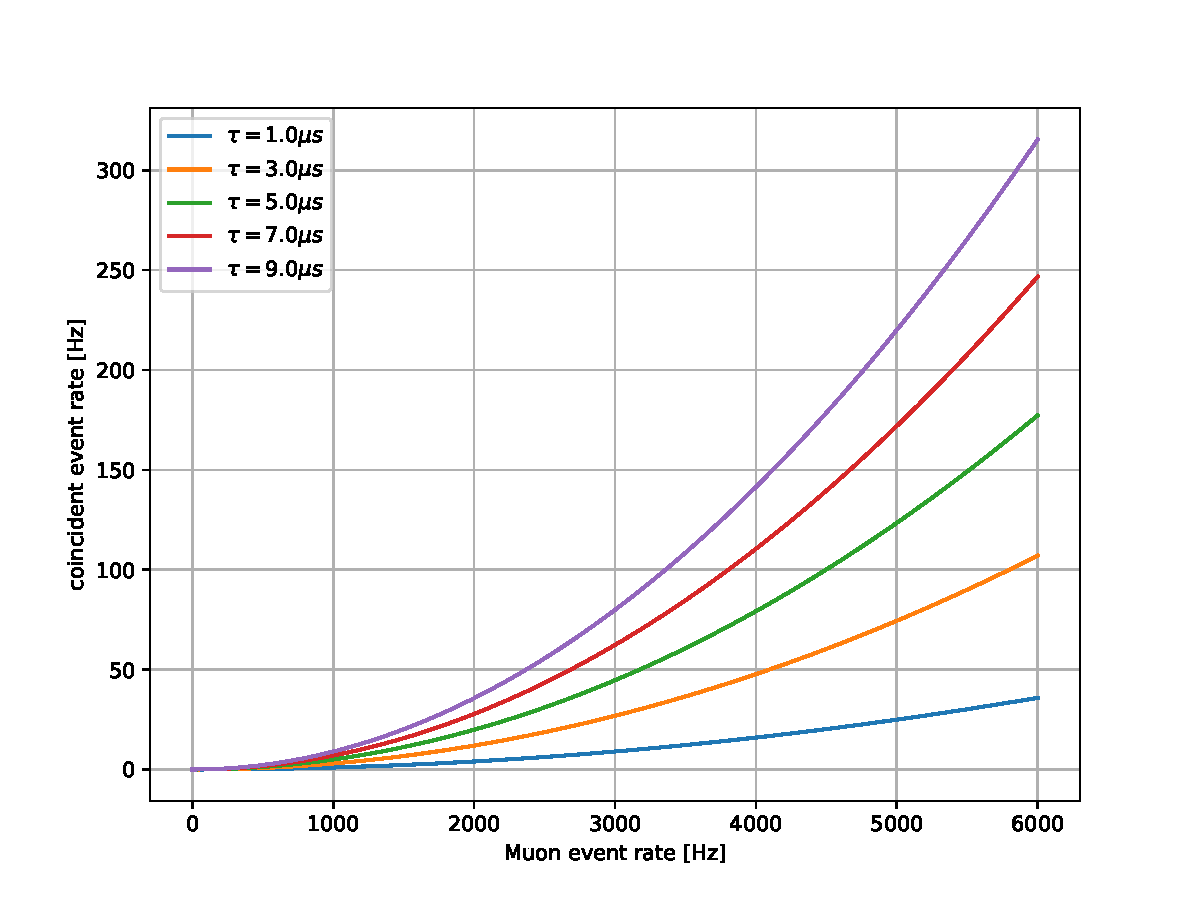
\includegraphics[width=0.7\textwidth]{Plots/coincidence_rate_poisson.pdf}
    \caption{A graph showing the relation between the muon event rate and the corresponding event rate assuming a poisson distributed muon event rate.}
    \label{fig:coin_rate_rate}
\end{figure}

In order to put this into a meaningful context, a relation of the muon event rate and their corresponding energy is extracted from a monte carlo simulation.
With this data describing a step function $rate(energy)$, equation~\ref{eq:multi_rate} can be used to visualize the relation between the muon energy and their 
corresponding rate of coincident events. Equivalent calculations are made on a zenith angle spectrum, for which the data is extracted from the same set of monte 
carlo data. Both of these distributions, along with the corresponding intervals, in which the coincidence probability exceeds \SI{0.1}{\percent}, are shown in 
figure~\ref{fig:coin_rate_combined}.

\begin{figure}[ht]
    \centering
    \begin{subfigure}[b]{\textwidth}
        \centering
        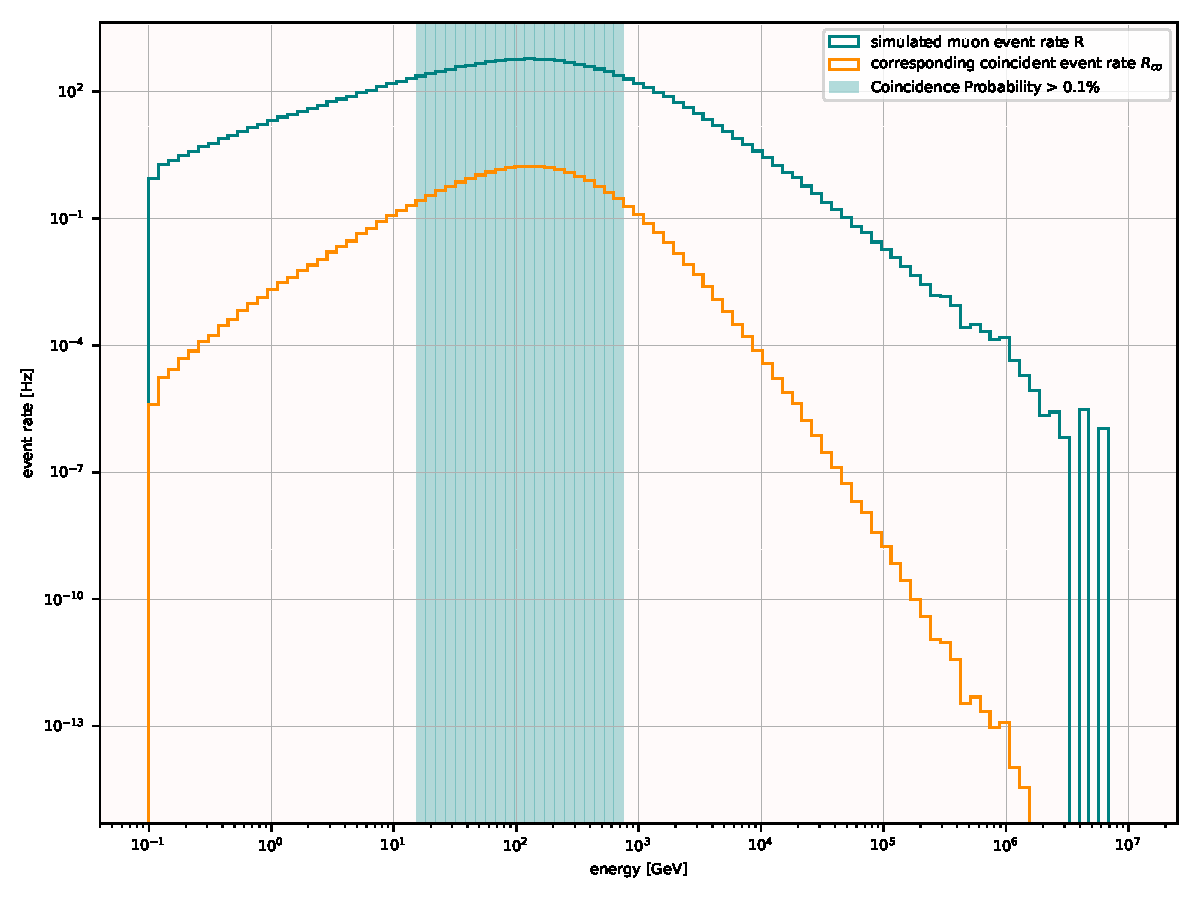
\includegraphics[width=0.7\textwidth]{Plots/coincidence_rate_energy.pdf}
    \end{subfigure}
    \vspace{1em} % Optional vertical space between the plots
    \begin{subfigure}[b]{\textwidth}
        \centering
        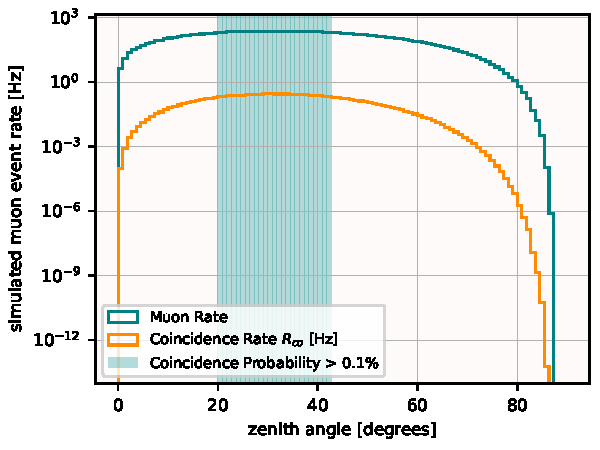
\includegraphics[width=0.7\textwidth]{Plots/coincidence_rate_zenith.pdf}
    \end{subfigure}
    \caption{Comparisons of the muon event rate and corresponding coincident event rate on energy and zenith angle spectra.}
    \label{fig:coin_rate_combined}
\end{figure}


Both histograms only show the theoretical coincidence event rate for a fixed trigger window $\tau$. However, diffrent triggers have diffrent readout windows, which 
can significantly change the probability of a coincident event. Treating the readout window as a variable, the coincident event probabilities can be visualized in 
a heat map to get a look at the effects of differing readout windows, as shown in figure~\ref{fig:heatmaps_combined}.

\begin{figure}[ht]
    \centering
    \begin{subfigure}[b]{\textwidth}
        \centering
        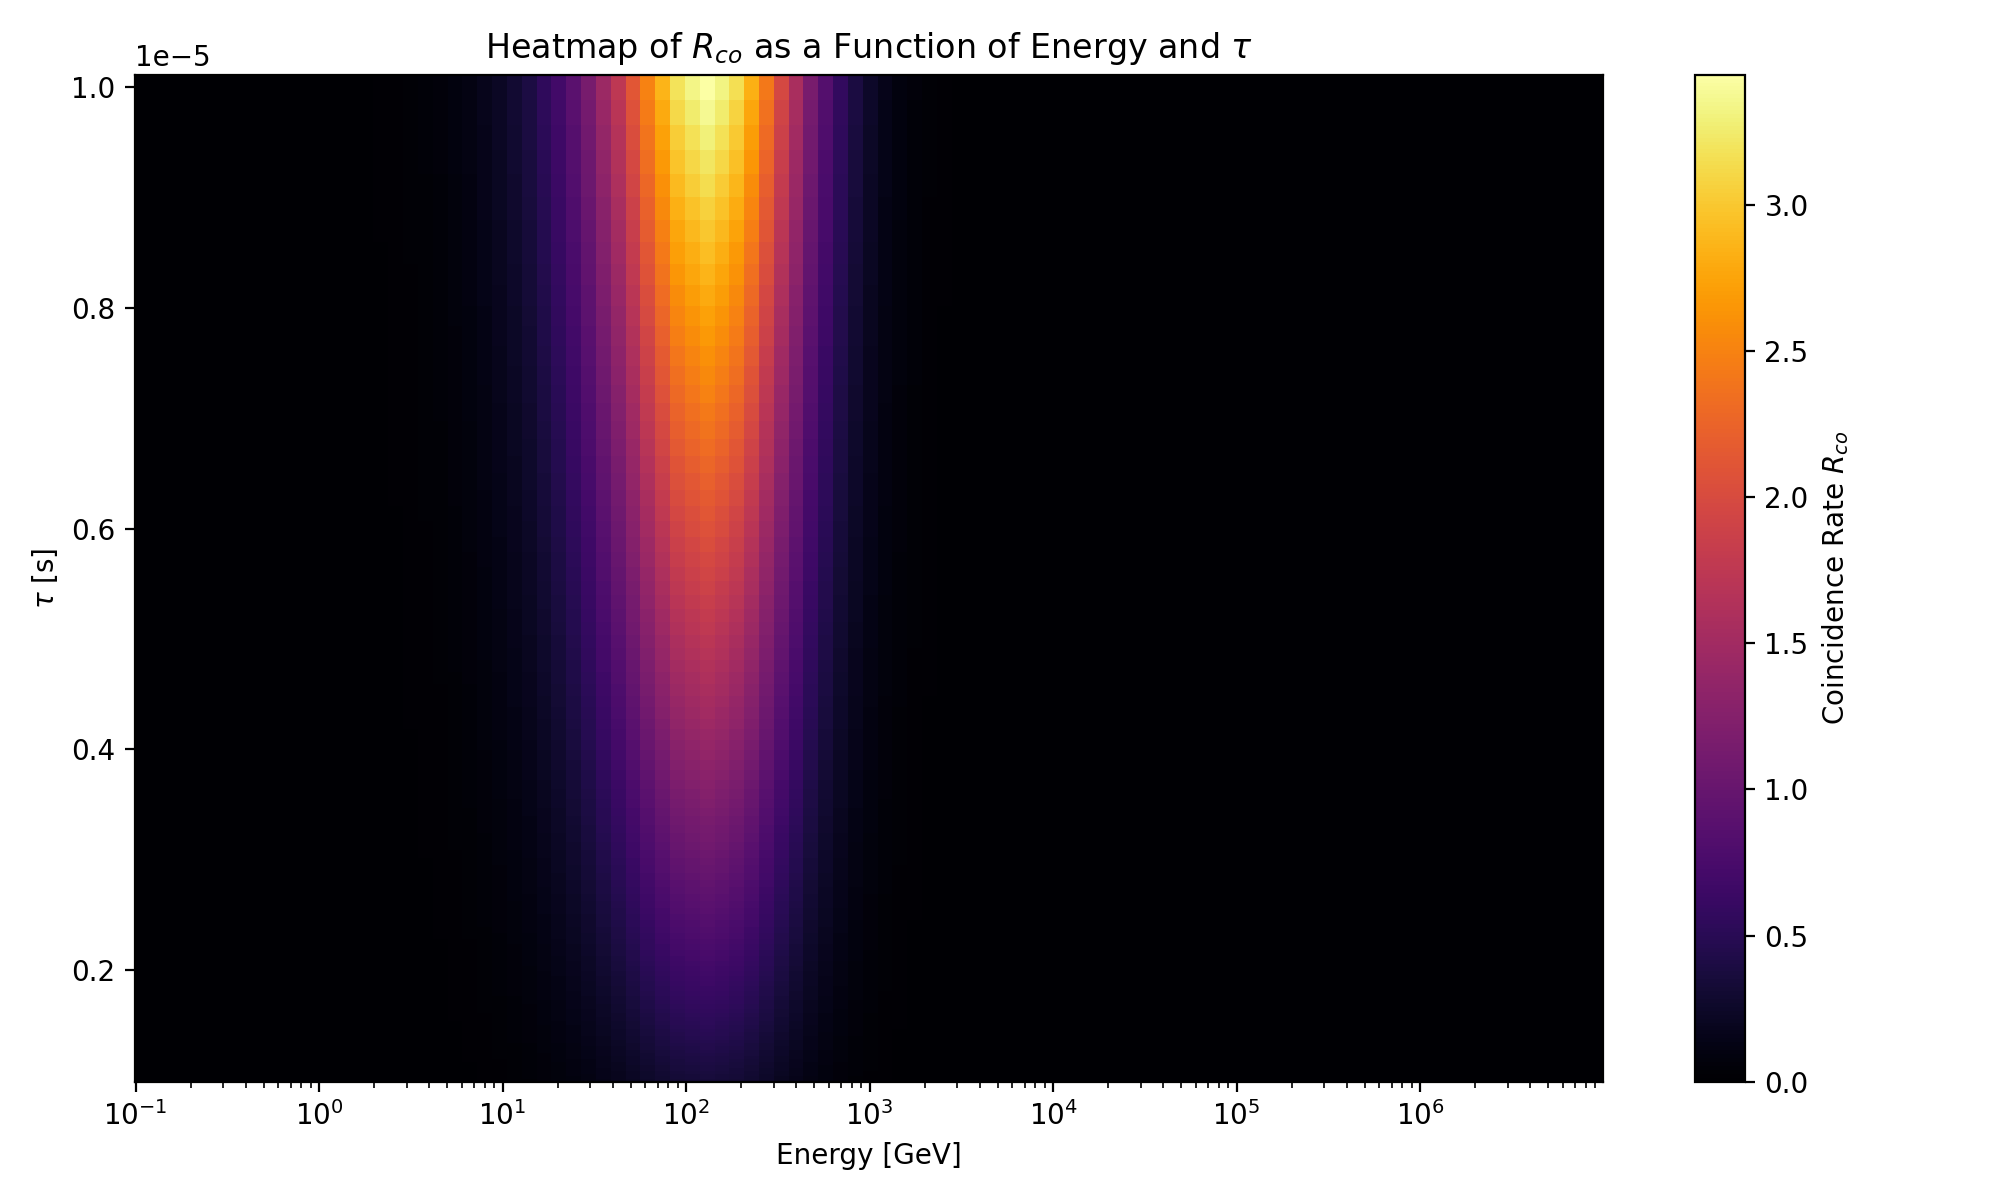
\includegraphics[width=0.7\textwidth]{Plots/heatmap_energy.png}
    \end{subfigure}
    \vspace{1em} % Optional vertical space between the plots
    \begin{subfigure}[b]{\textwidth}
        \centering
        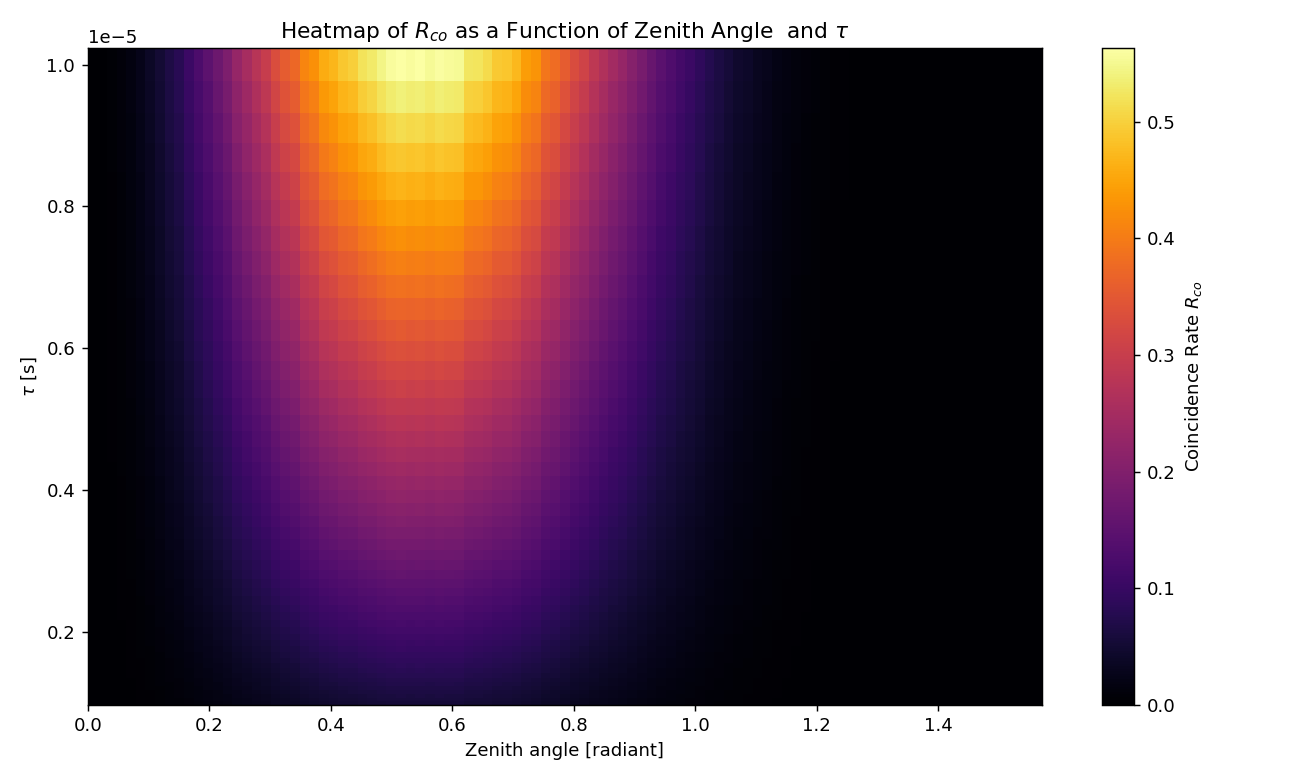
\includegraphics[width=0.7\textwidth]{Plots/heatmap_zenith.png}
    \end{subfigure}
    \caption{Prototypes of the heatmaps for energy and zenith angle spectra.}
    \label{fig:heatmaps_combined}
\end{figure}

\section{Analysis of the Fixed Rate Trigger}

As mentioned in section~\ref{sec:daq}, the FRT has a comparatively large readout window of \SI{10}{ms}. The result of this is that one \textit{event} contains 
a substantial amount of DOM hits. Since the average muon rate in IceCube is around \num{2200}\unit{Hz}, there is a significant likelihood, that any \textit{event}
contains physically significant signals. Other than muon events, there might be neutrino events as well as other possible atmospheric or astrophysical signals 
being measured in a given readout window of the FRT. However, a major fraction of the signals detected by the FRT is expected to be noise. 
(wie gibt man den Datensatz an, gibt es da einen standart?). The subsequent analysis is an attempt to extract knowledge about the composition of the signals 
measured by FRT and to possibly use them to better understand coincident events in IceCube.\\

The first step breaking down the FRT's data is to inspect the kind of signals detected in a singular DOM hit. In accordance with the description of 
\textit{subevents} in \ref{sec:daq}, a python script is used to filter out the corresponding signals (detaillierter~?). Depicted in 
figure~\ref{fig:frt_mu_sub_comp_1} is a comparison of the unfiltered and filtered signals detected over the course of \num{5035} \textit{events}. Most notably, 
the two distributions show a 
general similarity between them. As expected, there are substantially more unfiltered signals than filtered signals, showing that there are infact signals 
being filtered. The expectation would be to see a clear shift towards higher 
charge values in distribution of filtered signals, based on the idea that signals which stem from astrophysical or atmospheric sources would carry higher energy 
than noise signals. The observation does not quite match this expectation of clearly distinguished distributions. 

\begin{figure}[H]
    \centering
    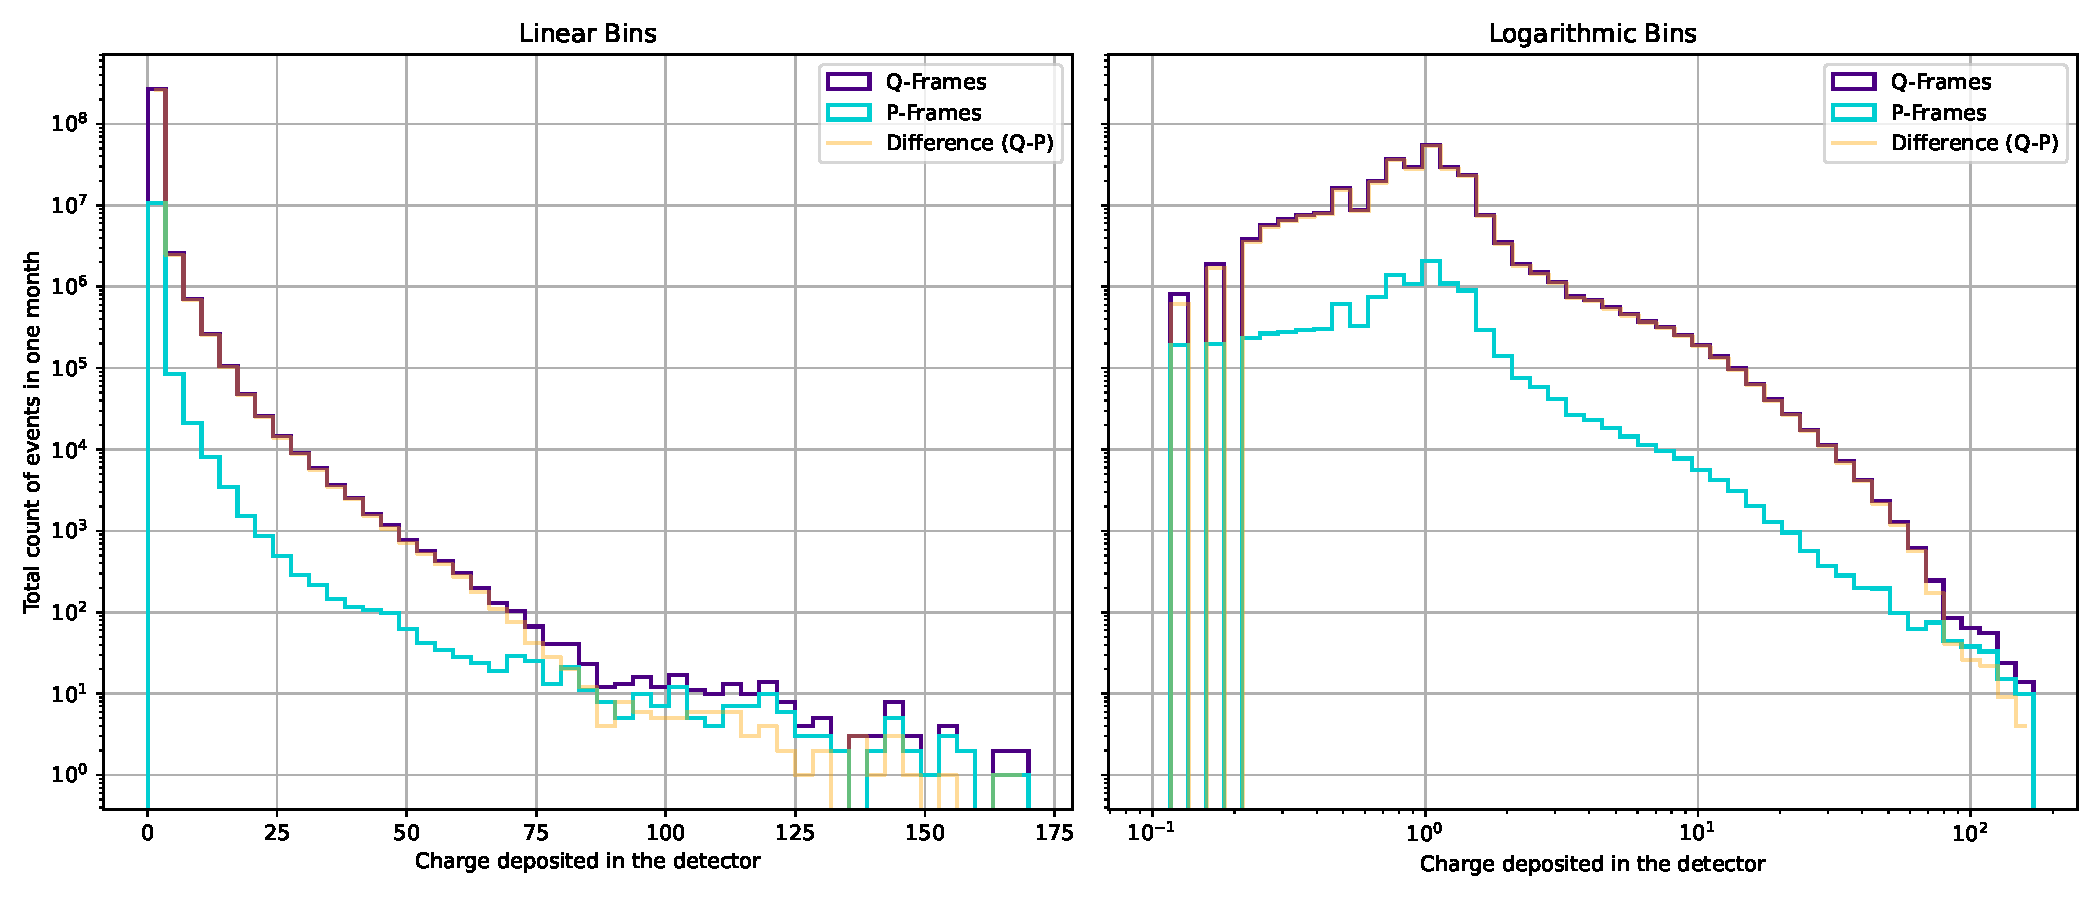
\includegraphics[width=\textwidth]{Plots/q_p_comp.pdf}
    \caption{A comparison between the counts of all Signals and physics signals.}
    \label{fig:frt_mu_sub_comp_1}
\end{figure}

To gather a deeper understanding of the signals measured and how they might be filtered, a comparison of mean charges for the individual DOMs is created. 
Figure~\ref{fig:mean_dom_charge_pq} shows the mean charge per DOM hit of every individual DOM over \num{5035} \textit{events}. 
The mean charges are quite evenly distributed throughout the DOMs, with the exeption of the DOM (61,13), which shows an unusually high mean charge of 
\num{5.08}~\unit(PE). Another notable characteristic of the filtered signals, although not easily visible, is the slightly higher mean charge around the 35th OM. 
%(values)
Other than that, there are no immediately visible anomalies in the general pattern of mean charges throughout the detector. 

\begin{figure}[H]
    \centering
    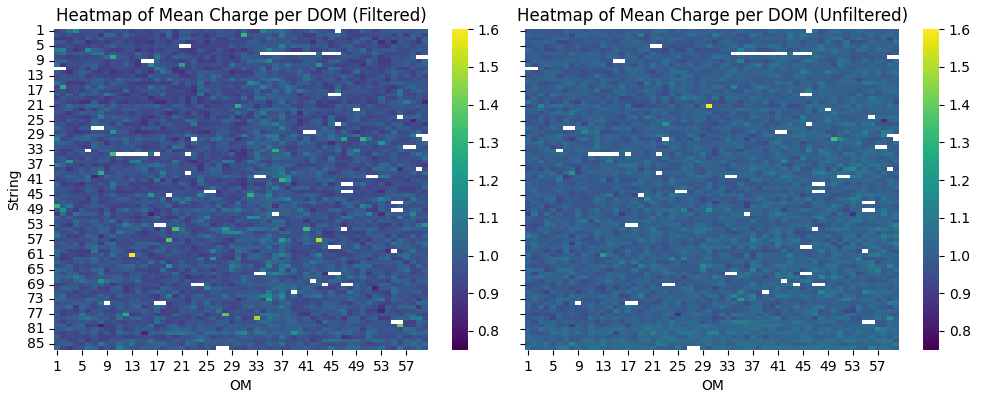
\includegraphics[width=\textwidth]{Plots/mean_charge_all_dom.png}
    \caption{The mean charge of every individual DOM for filtered and unfiltered signals.}
    \label{fig:mean_dom_charge_pq}
\end{figure}

While the analysis of mean charges over time allow for the possible detection of general anomalies or trends in the DOMs, it does not provide clear indicators for 
significant signals without additional information. When detecting a substantial signal, the expected behavior is a clear spike in the charge over function. 
Measuring these signals frequently might therefore have a visible impact on the standard deviation of the measured charge. The comparison of filtered and unfiltered 
signals regarding the mean charge values and their standard deviation is shown in figure~\ref{fig:mean_std_comp}.

\begin{figure}[H]
    \centering
    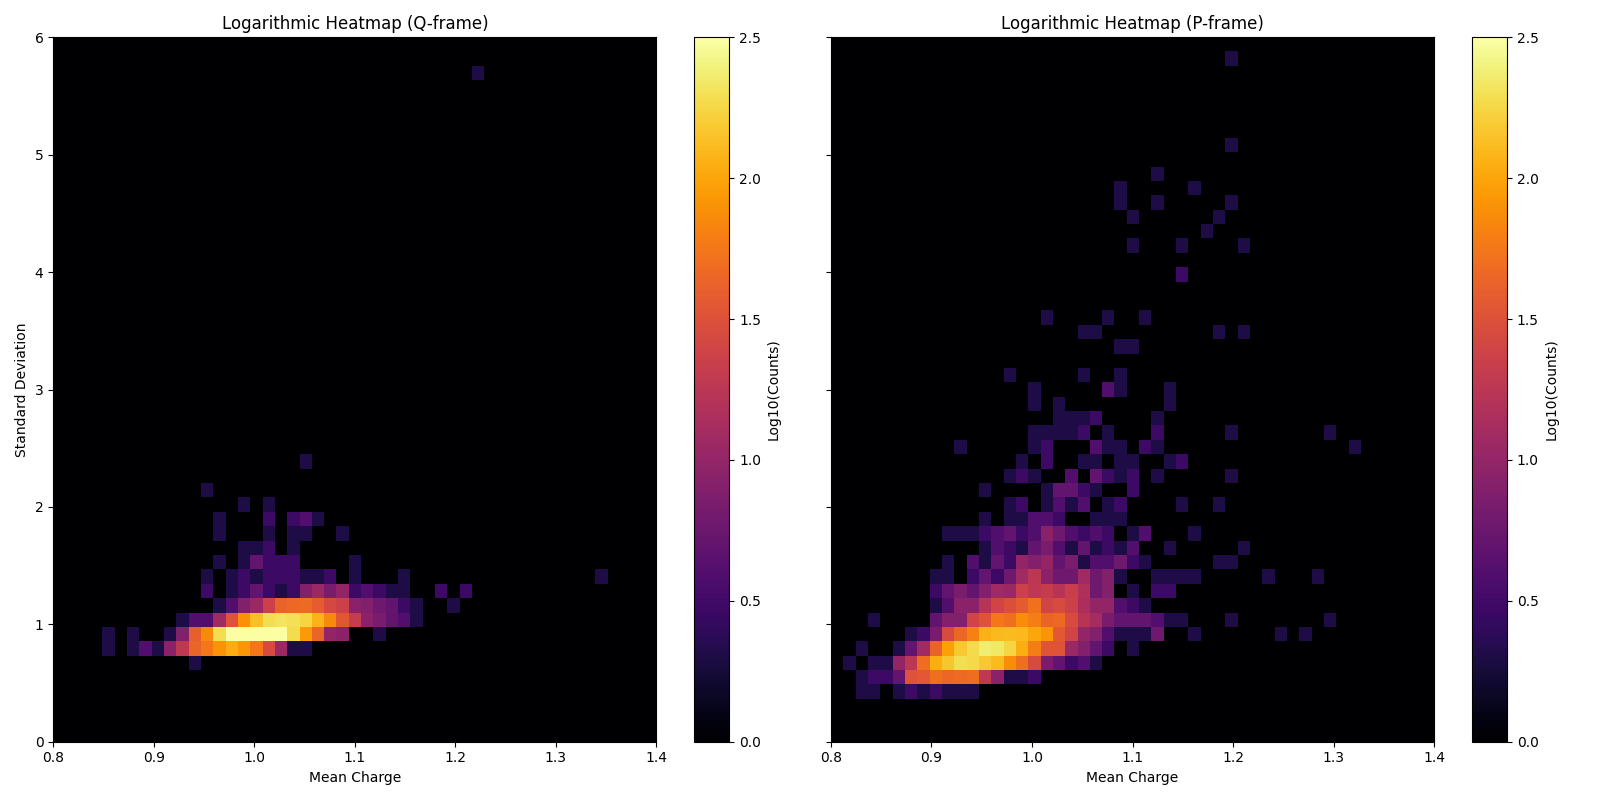
\includegraphics[width=0.9\textwidth]{Plots/mean_std_charge.png}
    \caption{A Comparison of the mean charge and standard deviation for filtered and unfiltered signals.}
    \label{fig:mean_std_comp}
\end{figure}

Clearly visible is the substantially larger spread of charges in the filtered signals. While the mean charges do not differ significantly from those of the 
unfiltered signals, there is a notable tendency towards larger deviation from the mean charge for the filtered signals. 
While this tendency suggests multiple measurements of high energy signals in those DOMs which show these high standard variations, the observation that the vast 
majority of filtered signals are clustered around a similar mean charge and standard deviation, as seen in figure~\ref{fig:mean_std_hist}, leads to the speculation 
that the filtered signals might still contain a considerable amount of noise.

\begin{figure}[H]
    \centering
    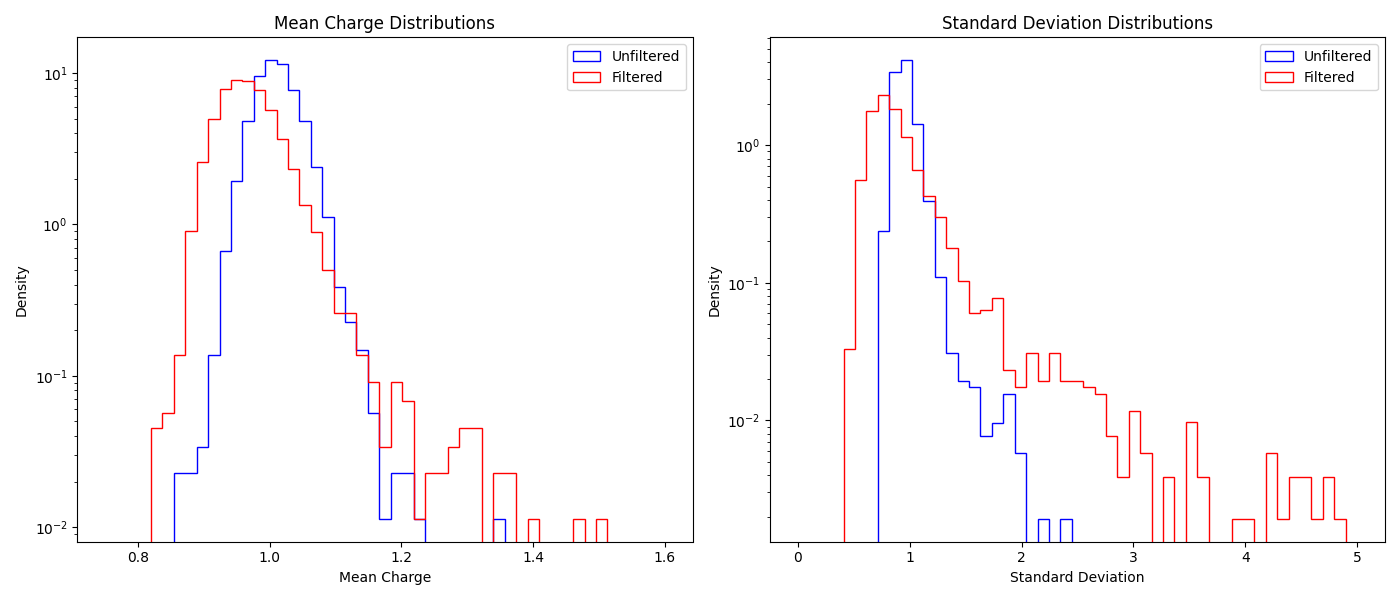
\includegraphics[width=0.9\textwidth]{Plots/qp_mean_std_comparison_histograms.png}
    \caption{An Individual Comparison of the mean charge and standard deviation.}
    \label{fig:mean_std_hist}
\end{figure}

Another interpretation could be, that the majority of signals of interest have infact comparatively low energies, leading to an average charge per DOM hit of 
just below \num{1}\unit{PE}. A disirable characteristic to observe would have been a certain charge threshold, below which none of the filtered signals 
would be observed. This would result in a strict condition that could be applied to certain triggers or other software. However, this is not the case. 

% further analysis:
% 1. charge over time p and q
% 2. charge over time in single events
% 3. filtermask with different plots
% 4. filter event candidates via simple algorithm -> clusters

Thus far, the signals detected by the FRT have been analyzed with a focus on individual DOM behavior. Another important property to examine is the charge per 
time function within singular events. Since one event accompasses a time window of \SI{10}{\milli\second}, a substantial amount of signals should be 
recorded for one event. This charge distribution over time for the entire detector is shown in figure~\ref{fig:charge_time_1}.

\begin{figure}[ht]
    \centering
    \begin{subfigure}[b]{\textwidth}
        \centering
        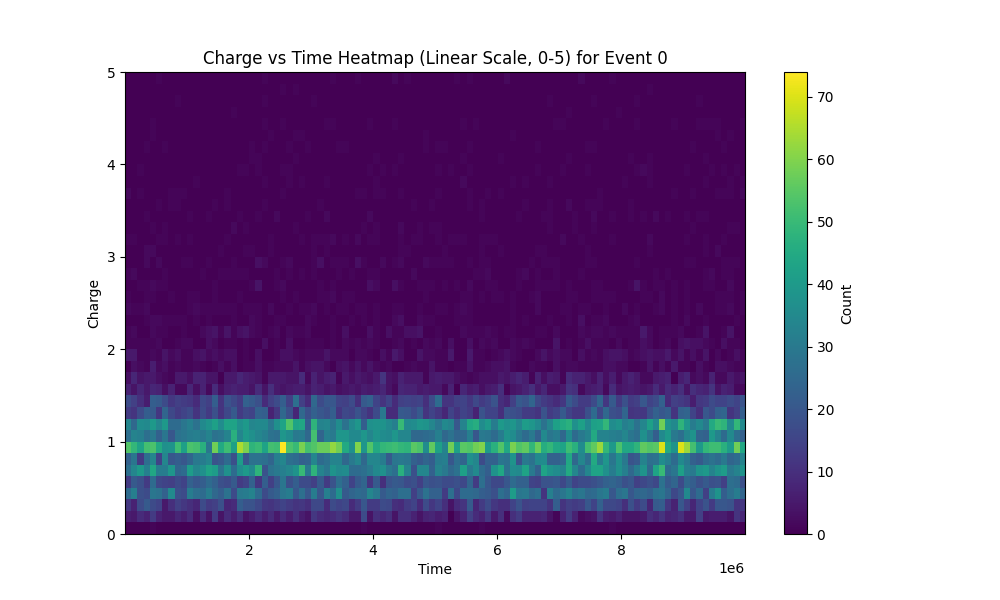
\includegraphics[width=0.7\textwidth]{Plots/charge_time_1_lin.png}
    \end{subfigure}
    \vspace{1em} % Optional vertical space between the plots
    \begin{subfigure}[b]{\textwidth}
        \centering
        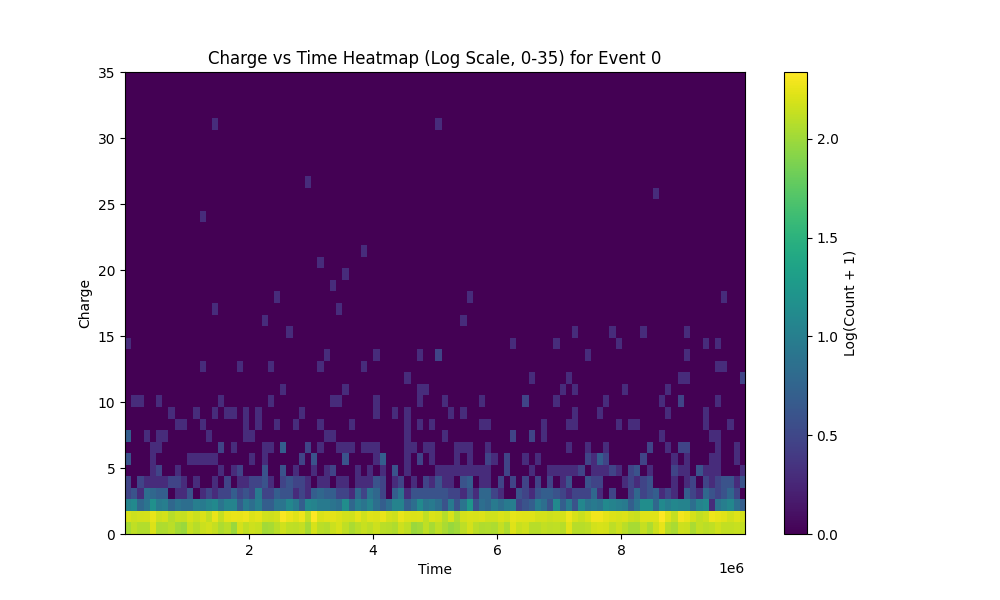
\includegraphics[width=0.7\textwidth]{Plots/charge_time_1_log.png}
    \end{subfigure}
    \caption{charge per time within one event (entire detector).}
    \label{fig:charge_time_1}
\end{figure}

Due to the long readout window of the FRT, the distribution of charge per time is visibly even during the event and does not differ significantly between 
individual events. This leads back to the inspection of the filtered signals. These signals are clustered in subevents, which should have significantly
more distinct features with regards to their corresponding charge over time measurements. From the previous analysis however, these filtered subevents 
have been shown to contain a substantial amount of signals with comparatively low charges. As a visual comparison, two subevents with comparatively high 
total charge are shown next to two average subevents. 

\begin{figure}[h!]
    \centering
    % First row
    \begin{subfigure}[t]{0.49\textwidth}
        \centering
        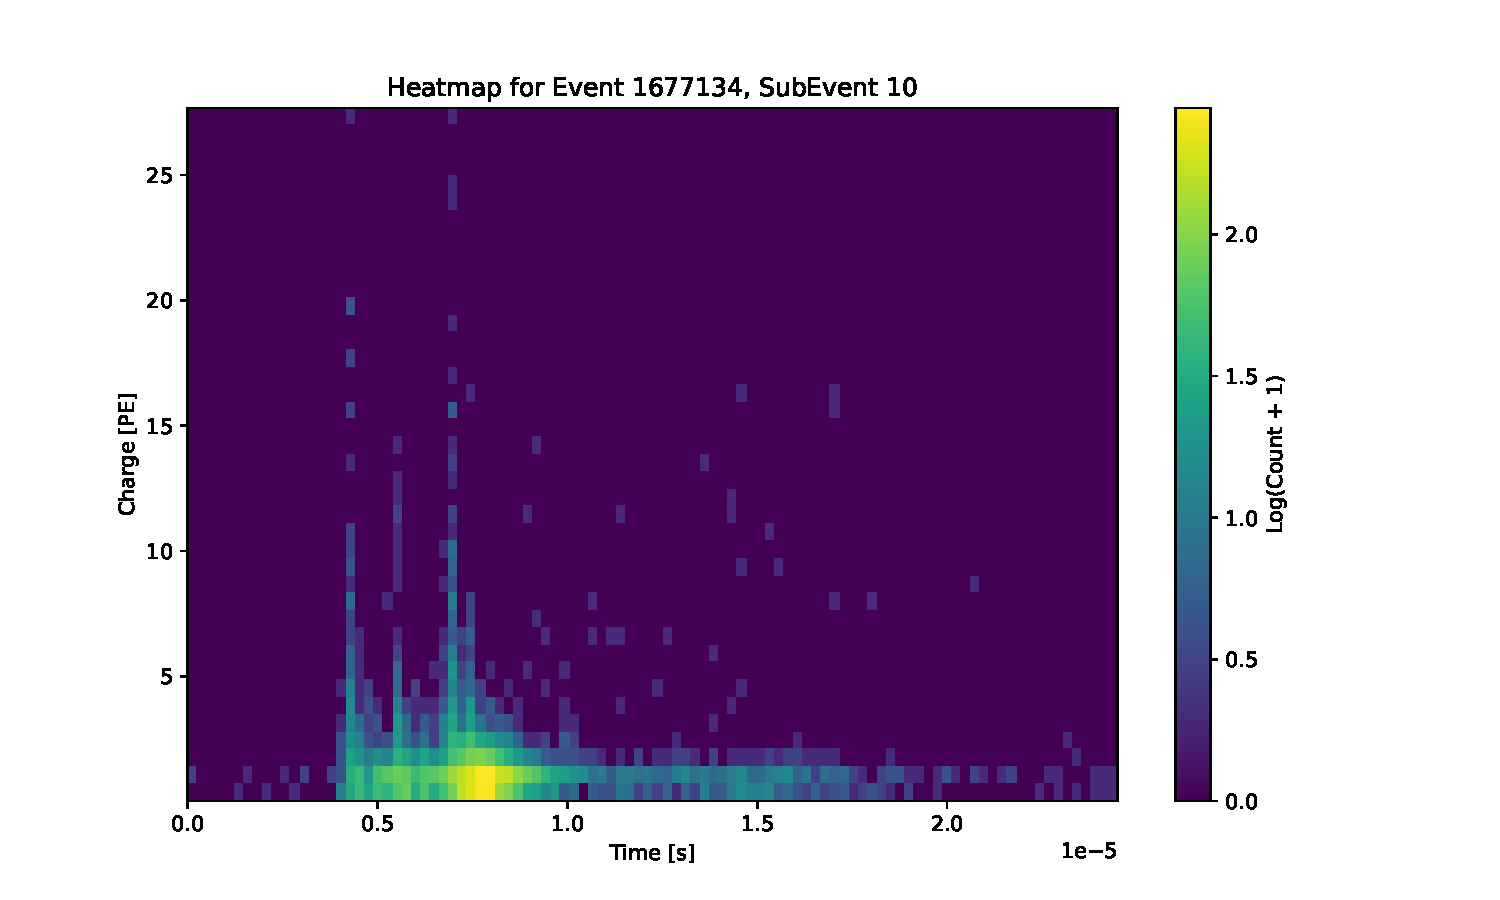
\includegraphics[width=\textwidth]{Plots/heatmap_subevent_triple_high.pdf}
        \caption{SubEvent 1: Description here.}
        \label{fig:subevent1}
    \end{subfigure}
    \hfill
    \begin{subfigure}[t]{0.49\textwidth}
        \centering
        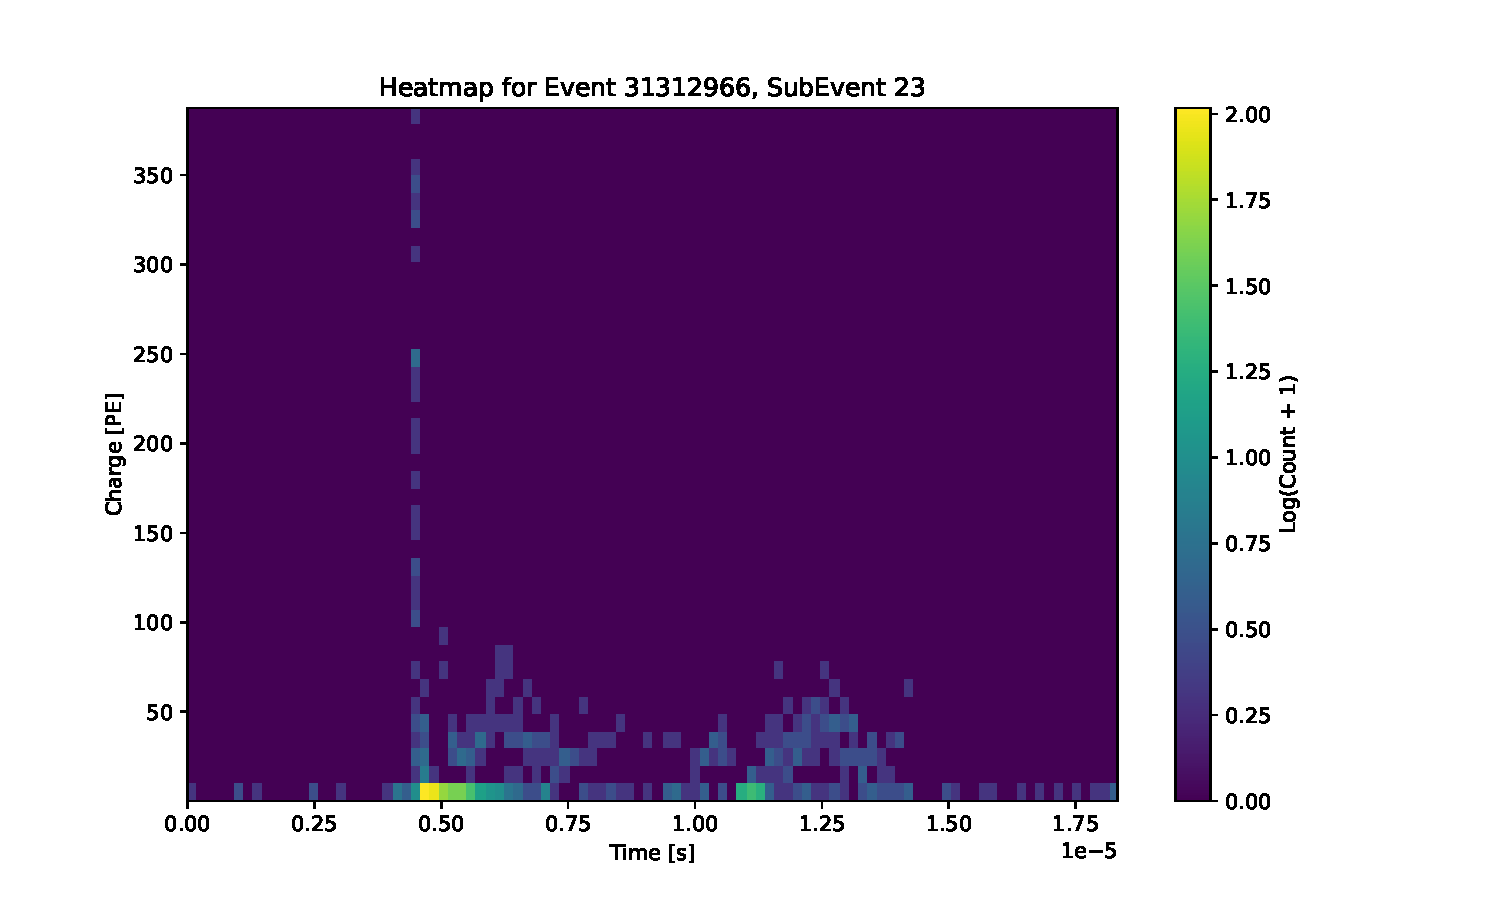
\includegraphics[width=\textwidth]{Plots/heatmap_subevent_double_high.pdf}
        \caption{SubEvent 2: Description here.}
        \label{fig:subevent2}
    \end{subfigure}
    
    % Second row
    \vspace{0.5cm} % Adjust vertical spacing as needed
    \begin{subfigure}[t]{0.49\textwidth}
        \centering
        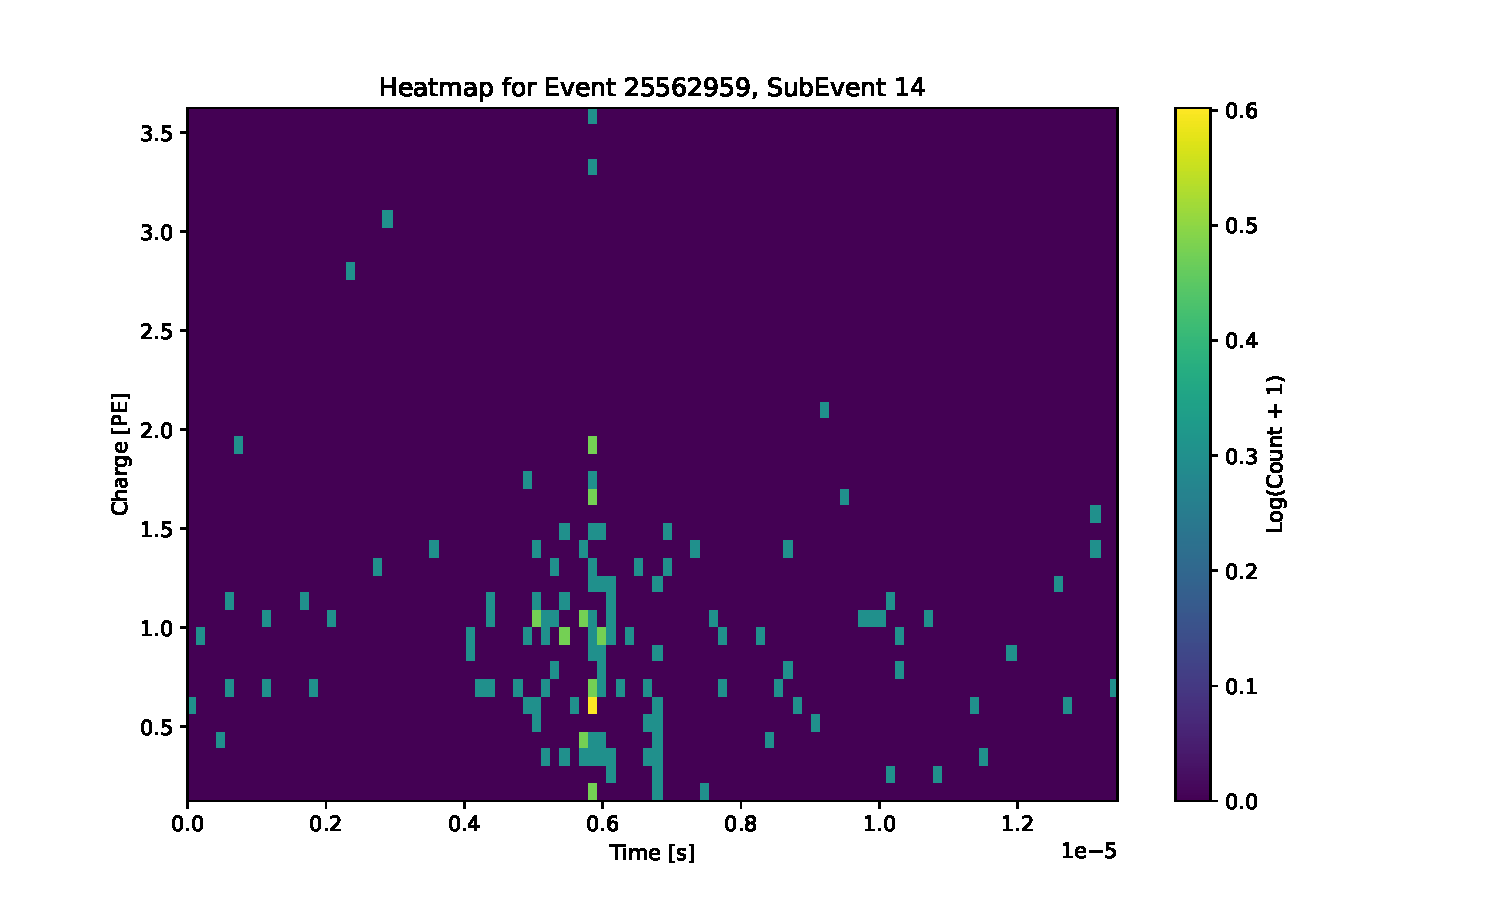
\includegraphics[width=\textwidth]{Plots/heatmap_subevent_random_1.pdf}
        \caption{SubEvent 3: Description here.}
        \label{fig:subevent3}
    \end{subfigure}
    \hfill
    \begin{subfigure}[t]{0.49\textwidth}
        \centering
        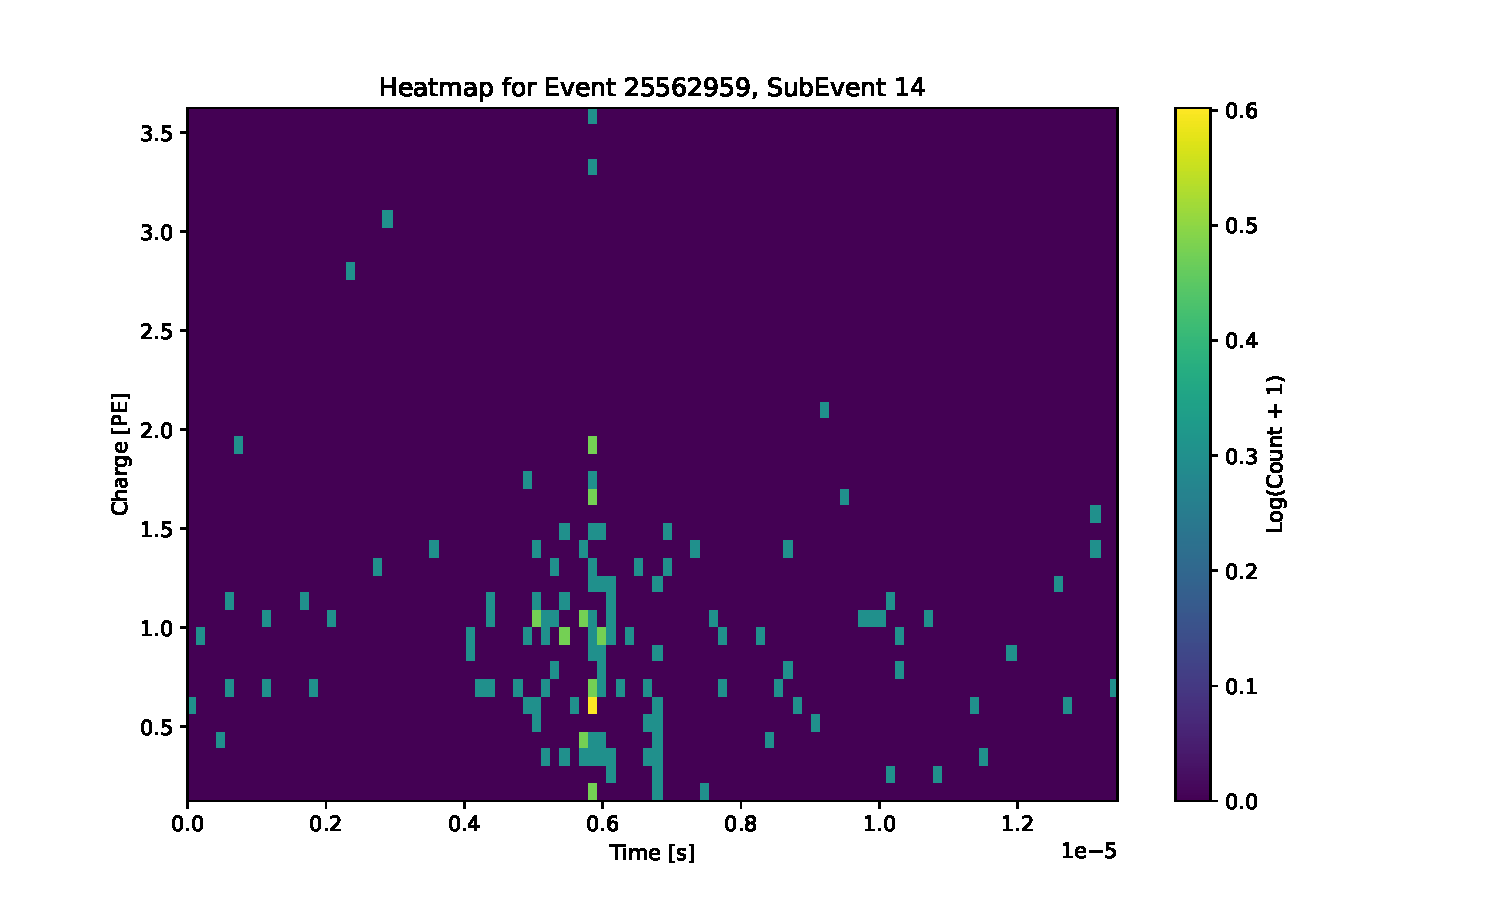
\includegraphics[width=\textwidth]{Plots/heatmap_subevent_random_1.pdf}
        \caption{SubEvent 4: Description here.}
        \label{fig:subevent4}
    \end{subfigure}

    % Main caption for the figure
    \caption{Comparison of heatmaps for four different SubEvents. }
    \label{fig:subevent_charge_time}
\end{figure}

While the visual difference between these subevents of vastly differing mean charge is immediately evident, a specificly interesting characteristic can be 
observed for the subevents 1 and 2. These subevents show multiple peaks of charge and signal count within their individual time frame. As these features
might be indicators for coincident events, these structures are analyzed in detail. 

There are a variety of possible approaches for identifying possible coincident event candidates. In the subsequent analysis, the python function $\text{find\_peaks}$ 
from 
the scipy library is used. Singular events are characterized by a combindation of the charge values, as well as the signal counts on a time scale within the time 
frame of a subevent. This time frame is divided into \num{100} equally spaced bins. For each bin, the sum of the charges ($Q_P$) measured within is calculated, 
as well as the total counts ($N_P$) within in the bin. These projections are combined into a weighted projection ($W_P$)

\begin{equation}
    W_P = \alpha\cdot Q_P +  \beta\cdot N_P\,
\end{equation}

where the weights \alpha and \beta are calculated via the equation

\begin{align}
    \alpha &= \frac{M_N + \sigma_N^2}{(M_C + \sigma_C^2) + (M_N + \sigma_N^2)} \\
    \beta &= 2\frac{M_C + \sigma_C^2}{(M_C + \sigma_C^2) + (M_N + \sigma_N^2)}
\end{align}


where $(M_C)$ and ($M_N$) represent the sums of the charge and count projections, respectively, and ($\sigma_C^2$) and ($\sigma_N^2$) denote their variances. 
These weights ensure that both the magnitude and variability of the projections are accounted for in the weighted projection. 

$W_P$ is then used as the function for which the $\text{find\_peaks}$ method is applied. This method takes multiple parameters, which were determined empirically 
based on a variety of subevent samples. These parameters are shown in table~\ref{tab:peak_parameters} along with their respective description.


\begin{table}[h!]
    \centering
    \begin{tabular}{|l|l|p{7cm}|}
    \hline
    \textbf{Parameter} & \textbf{Value} & \textbf{Description} \\ \hline
    Prominence & 5 & The minimum vertical distance a peak must stand out relative to its neighboring valleys. This ensures that only significant peaks are detected. \\ \hline
    Height & Dynamic (\(5\%\) baseline + \(1.5 \cdot \sigma\)) & The minimum value a peak must reach to be considered valid. This threshold is calculated dynamically based on the signal's baseline noise (5th percentile) and its standard deviation (\(\sigma\)). \\ \hline
    Distance & 4 bins & The minimum number of bins required between consecutive peaks to ensure they are sufficiently separated and not falsely grouped. \\ \hline
    \end{tabular}
    \caption{Final parameters used for peak detection in the weighted projection of charge and count data.}
    \label{tab:peak_parameters}
\end{table}


The workings of this method are visualized for an example subevent in figure~\ref{fig:find_peaks}

\begin{figure}[ht]
    \centering
    \begin{subfigure}[b]{\textwidth}
        \centering
        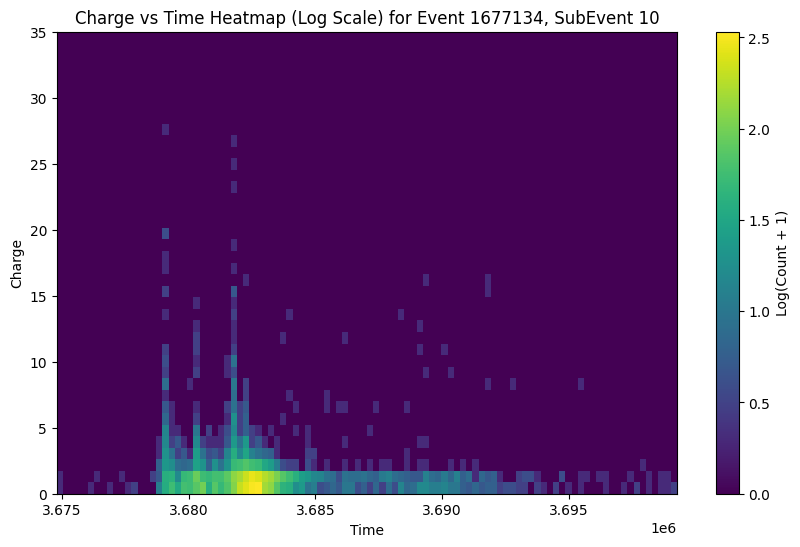
\includegraphics[width=0.7\textwidth]{Plots/peak_heat_1.pdf.png}
    \end{subfigure}
    \vspace{1em} % Optional vertical space between the plots
    \begin{subfigure}[b]{\textwidth}
        \centering
        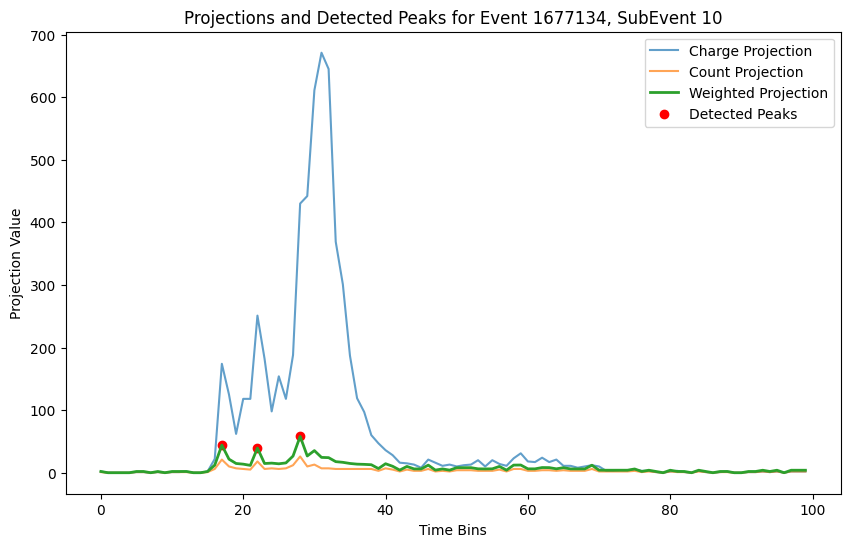
\includegraphics[width=0.7\textwidth]{Plots/peak_plot_1.png}
    \end{subfigure}
    \caption{caption}
    \label{fig:find_peaks}
\end{figure}

While this method seems to be working decently well for subevents with large enough charges, it struggles with those subevents that lack distinctly defined 
features. With the current set of parameters, the following results are concluded:

\begin{align}
    total subevents &= 137342 \\
    \frac{N(multiple peaks)}{N(any peaks)} &= 0.54 \\
    \frac{N(any peaks)}{N(total)} &= 0.85
\end{align}

The evaluation of these results is discussed in the subsequent chapter~\ref{chap:discussion}










